\documentclass{VUMIFPSbakalaurinis}
\usepackage{algorithmicx}
\usepackage{algorithm}
\usepackage{algpseudocode}
\usepackage{amsfonts}
\usepackage{amsmath}
\usepackage{bm}
\usepackage{caption}
\usepackage{color}
\usepackage{float}
\usepackage{graphicx}
\usepackage{listings}
\usepackage{subfig}
\usepackage{wrapfig}
\usepackage{array}
\usepackage[table]{xcolor}

% Titulinio aprašas
\university{Vilniaus universitetas}
\faculty{Matematikos ir informatikos fakultetas}
\department{Programų sistemų katedra}
\papertype{1 Laboratorinis darbas}
\title{Smulkių darbų programėlė}
\author{Šarūnas Bagdonavičius}
\secondauthor{Andrius Bureika}
\thirdauthor{Juras Jankauskas}
\fourthauthor{Odeta Kizytė}
\supervisor{dr. Vytautas Valaitis}
\date{Vilnius – \the\year}

% Nustatymai
% \setmainfont{Palemonas}   % Pakeisti teksto šriftą į Palemonas (turi būti įdiegtas sistemoje)
\bibliography{bibliografija}
\setcounter{tocdepth}{3}

\begin{document}
\maketitle
\tableofcontents

\sectionnonum{Įvadas}
Šiame dokumente pateikiami reikalavimai, struktūrinis dalykinės srities modelis bei užduočių vykdymo scenarijai mobiliajai programėlei „Help4Help“. Reikalavimai išskirstyti į funkcinius ir nefunkcinius. Funkciniai reikalavimai išskirstyti į pagrindinius ir šalutinius, o nefunkciniai reikalavimai išskirstyti į sisteminių interfeisų, veikimo, diegimo, aptarnavimo ir priežiūros, tiražuojamumo, apsaugos, juridinius bei pranešimų formulavimo reikalavimus. Darydami darbą rėmėmės ICONIX procesu.

\section{Reikalavimai}
Šiame skyriuje pateikiami reikalavimai mobiliajai programėlei „Help4Help“.
\subsection{Funkciniai reikalavimai}
Šiame poskyryje išskiriami funkciniai reikalavimai sistemai.
\subsubsection{Pagrindiniai funkciniai reikalavimai}
Šiame skirsnyje pateikiami pagrindiniai funkciniai reikalavimai sistemai.
\subsubsubsection{Naudotojo sąsajos funkcijos}
\begin{itemize}
	\item \textbf{FR1} Registruotis sistemoje (privalomi duomenys: el. pašto adresas, slaptažodis, vardas, pavardė, telefono numeris).
	\item \textbf{FR2} Prisijungti prie sistemos (privalomi duomenys: el. pašto adresas, slaptažodis).
	\item \textbf{FR3} Atnaujinti savo duomenis (pasirinktinai: el. pašto adresas, slaptažodis, gyvenamosios vietos adresas, telefono numeris).
	\item \textbf{FR4} Prašyti priminti užmirštą slaptažodį.
	\item \textbf{FR5} Atsijungti nuo sistemos.
	\item \textbf{FR6} Pateikti pagalbos prašymo užklausą
	\item \textbf{FR7} Atlikti esamų darbų paiešką (sąrašą surikiuoti pagal pasirinktus kriterijus ar kategorijas).
	\item \textbf{FR8} Peržiūrėti esamų darbų sąrašą.
	\item \textbf{FR9} Pasirinkti atlikti darbą.
	\item \textbf{FR10} Patvirtinti atliekamą darbą.
	\item \textbf{FR11} Atšaukti pasirinktą darbą.
	\item \textbf{FR12} Įvertinti kitą naudotoją.
	\item \textbf{FR13} Peržiūrėti kito naudotojo paskyrą.
	\item \textbf{FR14} Peržiūrėti individualizuotus darbų pasiūlymus (darbų pasiūlymai teikiami atsižvelgiant į jau prieš tai atliktus darbus).
	\item \textbf{FR15} Peržiūrėti atilktų darbų istoriją.
	\item \textbf{FR16} Peržiūrėti atsiskaitymų istoriją.
	\item \textbf{FR17} Peržiūrėti savo reitingą.
	\item \textbf{FR18} Peržiūrėti naudotojų reitingų lentelę(lentelė pateikiama išrikiavus naudotojus mažėjimo tvarka pagal didžiausią reitingą).
	\item \textbf{FR19} Naudotojo sąsajos funkcijas įgyvendina mobili aplikacija „Help4Help“.
\end{itemize}

\subsubsubsection{Sistemos administratoriaus sąsajos funkcijos}
\begin{itemize}
	\item \textbf{FR20} Prisijungti prie sistemos (privalomi duomenys: el. pašto adresas ir slaptažodis).
	\item \textbf{FR21} Atsijungti nuo sistemos.
	\item \textbf{FR22} Sukurti naują vartotojo paskyrą duomenų bazėje.
	\item \textbf{FR23} Ištrinti vartotojo paskyrą iš duomenų bazės.
	\item \textbf{FR24} Pašalinti pagalbos prašymo užklausą iš sąrašo.
	\item \textbf{FR25} Patvirtinti naują naudotoją.
	\item \textbf{FR26} Pativrtinti atsiskaitymą.
	\item \textbf{FR27} Redaguoti naudotojo paskyros duomenis (pasirinktinai: el. pašto adresas, slaptažodis, vardas, pavardė, asmens kodas, gyvenamosios vietos adresas, telefono numeris).
	\item \textbf{FR28} Atsakyti į naudotojų klausimus.
	\item \textbf{FR29} Išsiųsti pranešimą naudotojams (privalomai: gavėjų el. pašto adresai, antrašė, pranešimo tekstas).
	\item \textbf{FR30} Peržiūrėti registruotų naudotojų sąrašą, jų prašymų užklausų pateikimo istorijas, atsiskaitymo istorijas.
	\item \textbf{FR31} Peržiūrėti kasdienį lankomumą.
	\item \textbf{FR32} Peržiūrėti naudotojų lokacijas.
	\item \textbf{FR33} Peržiūrėti naudotojų demografinės statistikos duomenis ( pvz.: pateikti pirkėjų dalį procentais pagal lytį).
	\item \textbf{FR34} Išsaugoti atsarginę duomenų kopiją.
	\item \textbf{FR35} Sistemos administratoriaus sąsajos funkcijas įgyvendina paties administratoriaus pasirinkti DB valdymo įrankiai.
\end{itemize}

\subsubsection{Šalutiniai funkciniai reikalavimai}
Šiame skirsnyje pateikiami šalutiniai funkciniai reikalavimai mobiliajai aplikacijai „Help4Help“.
\subsubsubsection{Aplikacijos navigacijos reikalavimai}
\begin{itemize}
	\item \textbf{FR36} Iš visų langų, prisijungus prie paskyros, galima atsidaryti navigacinį menių iš kurio galima nueiti į langus:
	\begin{itemize}
		\item Pagrindinis langas - kuriame iškart rodomas bendras darbų sąrašas;
		\item Mano paskyra - kuriame rodoma naudotojo paskyra;
		\item Mano darbai - kuriame rodomi naudotojo įkelti darbai ir darbai, kuriuos jis sutiko atlikti;
		\item Atlikti darbai - kuriame rodomas jau atliktų darbų sąrašas;
		\item Visų naudotojų reitingas;
		\item Prisijungimo langas (atsijungiant).
	\end{itemize}
	\item \textbf{FR37} Įsijungus applikaciją, naudotojas mato prisijungimo langą, kol neprisijungia arba neprisiregistruoja, vartotojas negali nueiti į kitus aplikacijos langus.
	\item \textbf{FR38} Iš visų naudotojų reitingo lango, galima nueiti į atskirų naudotojų paskytų langus
	\item \textbf{FR39} Iš darbų sąrašo, paspaudos ant specifinio darbo, galima patekti į to darbo aprašymo langą.
\end{itemize}

\subsubsubsection{Vartotojo registracija sistemoje}
\begin{itemize}
	\item \textbf{FR40} Prisijungdamas vartotojas užpildo šiuos duomenis:
	\begin{itemize}
		\item El. Pašto adresas,
		\item Slaptažodis
		\item Vardas,
		\item Pavardė,
		\item Telefono numeris.
	\end{itemize}
	\item \textbf{FR41} Tam, kad įvestas vartotojo el. pašto adresas būtų tinkamos formos, jis turi būti sudarytas iš abonento vardo, „@“ simbolio bei domeno adreso.
	\item \textbf{FR42} Slaptažodis privalo atitikti saugaus slaptažodžio reikalavimus. Saugiu slaptažodžiu laikomas toks, kuris yra sudarytas bent iš 8 simbolių, turi bent vieną skaitmenį ir raidę.
\end{itemize}

\subsubsubsection{Vartotojo prisijungimas sistemoje}
\begin{itemize}
	\item \textbf{FR43} Prisijungdamas vartotojas suveda email adresą ir slaptažodį.
	\item \textbf{FR44} Vartotojo įvesti duomenys (slaptažodis bei el. pašto adresas) turi buti sutikrinti su duomenimis, esančiais duomenų bazėje. Jei rastas atitikimas, vartotojas sėkmingai prijungiamas prie sistemos.
\end{itemize}

\subsubsubsection{Siūlomų darbų peržiūra}
\begin{itemize}
	\item \textbf{FR45} Darbų sąrašas gali būti rūšiuojamas pagal:
	\begin{itemize}
		\item artimiausią atstumą,
		\item atlygį,
		\item atlikimo datą.
	\end{itemize}
\end{itemize}

\subsubsubsection{Patvirtinimas atlikti darbą}
\begin{itemize}
	\item \textbf{FR46} Pagalbos teikėjas sutinka atlikti konkretų darbą.
	\item \textbf{FR47} Pagalbos prašantysis patvirtina arba atmeta paslaugos teikėją.
	\item \textbf{FR48} Po patvirtinimo pagalbos teikėjas gauna pranešimą, kad tiekėjas patvirtino jo ketinimą atlikti darbą
\end{itemize}

\subsubsubsection{Užsakymo apmokėjimas}
\begin{itemize}
	\item \textbf{FR49} Atsiskaitymai galimi tik virtualiais pinigais.
	\item \textbf{FR50} Atlikus darbą, teikėjas tai patvirtina ir laukia prašančiojo ivertinimo. Kai įvertinamas darbas, pinigai automatiškai pervedami iš pagalbos prašančiojo į pagalbos teikėjo sąskaitą.
\end{itemize}

\subsubsubsection{Pagalbos prašymo sukūrimas}
\begin{itemize}
	\item \textbf{FR51} Registruotas vartotojas sukuria paslaugos prašymą nurodydamas:
	\begin{itemize}
		\item Konkretų darbą
		\item Iki kada reikia atlikti konkretų darbą
		\item Užmokestį už atliktą darbą
	\end{itemize}
	\item \textbf{FR52} Visos kainos turi būti pateiktos virtualios valiutos vienetais.
\end{itemize}

\subsubsubsection{Užklausų pašalinimas}
\begin{itemize}
	\item \textbf{FR53} Jei nei vienas vartotojas nėra pradėjęs atlikti darbo, pagalbos prašantysis gali ištrinti savo sukurtą užklausą.
	\item \textbf{FR54} Jei jau pradėtas daryti, jis neberodomas darbo pasiūlymo sąraše.
\end{itemize}

\subsubsubsection{Slaptažodžio atkūrimas}
\begin{itemize}
	\item \textbf{FR55} Vartotojas, pamiršęs slaptažodį, gali jį pakeisti pasinaudodamas slaptažodžio atkūrimo forma. Formą sudaro el. pašto adreso įvedimo laukelis ir mygtukas slaptažodžio atkūrimo užklausai pateiki. Į laukelį įvedus sistemoje užregistruoto vartotojo el. pašto adresą ir paspaudus užklausos pateikimo mygtuką įvestuoju el. paštu išsiunčiamas laiškas su naudotojo slaptažodžiu.
\end{itemize}

\subsubsubsection{Pranešimas apie klaidą}
\begin{itemize}
	\item \textbf{FR56} Aptikus klaidą ar susidūrus su kitokia problema sistemoje vartotojas gali nesunkiai apie tai pranešti sistemos administratoriui naudodamasis pranešimo apie klaidą funkcija.
\end{itemize}

\subsection{Nefunkciniai reikalavimai}
Šiame poskyryje išskiriami nefunkciniai reikalavimai sistemai. 
\subsubsection{Sisteminių interfeisų reikalavimai}
\subsubsubsection{OS naudojimo reikalavimai}
\begin{itemize}
	\item \textbf{NFR1} Programų sistemos realizacijai neprivaloma naudoti specifinį OS.
	\item \textbf{NFR2} Mobiliajame įrenginyje turi būti įdiegta bet kuri iš Android (4.4 KitKat arba naujesnė versija) mobiliųjų operacinių sistemų.
\end{itemize}

\subsubsubsection{Sąveikos su Duomenų Baze reikalavimai}
\begin{itemize}
	\item \textbf{NFR3} Naudojama MySQL (pageidautina 5.6 arba naujesnes versijos) duomenų bazių valdymo sistema. Mobilioji aplikacija gauna duomenis iš „Microsoft Azure Web App“ internetinio serviso, kuris yra susietas su „Microsoft Azure Database“ MySQL 5.7 duomenų baze.
	\item \textbf{NFR4} DB turi lenteles „Vartotojas“, „Darbas“, kurioms įgalioti naudotojai gali sudaryti užklausas
\end{itemize}

\subsubsubsection{Darbo kompiuterių tinkluose reikalavimai}
\begin{itemize}
	\item \textbf{NFR5} Duomenys perduodami naudojant standartinį TCP/IP protokolą.
\end{itemize}

\subsubsubsection{Sąveikos su kitomis programomis reikalavimai}
\begin{itemize}
	\item \textbf{NFR6} Mobilioji aplikacija gauna informaciją apie vartotojo buvimo vietą iš mobiliojo įrenginio GPS sistemos.
\end{itemize}

\subsubsubsection{Programavimo aplinkos reikalavimai}
\begin{itemize}
	\item \textbf{NFR7} Mobilioji aplikacija kuriama Java programavimo kalba naudojant Android Studio.
	\item \textbf{NFR8} Mobiliosios aplikacijos internetinis servisas yra sukurtas naudojant XML-pagrindo informacijos keitimosi sistema ir naudoja HTTP protokolą.
\end{itemize}

\subsubsection{Veikimo reikalavimai}
\subsubsubsection{Vaizdavimo tikslumo reikalavimai}
\begin{itemize}
	\item \textbf{NFR9} Teksto užrašymui turi būti naudojama UTF-8 simbolių koduotė
	\item \textbf{NFR10} Darbo aprašymo antraštė – ne daugiau 25 simbolių.
	\item \textbf{NFR11} Darbo aprašymas – ne daugiau 500 simbolių.
	\item \textbf{NFR12} Atstumas nuo paslaugos atlikimo vietos – kilometrų tikslumų.
	\item \textbf{NFR13} Pinigai už paslaugą – centų tikslumu.
	\item \textbf{NFR14} Vartotojo prisijungimo vardas – ne daugiau 20 simbolių, specialieji simboliai neleidžiami
	\item \textbf{NFR15} Data turi būti vaizduojama formatu YYYY-MM-DD, kur YYYY – metai, MM – mėnuo, DD – diena.
	\item \textbf{NFR16} Laikas turi būti vaizduojamas minučių tikslumu, hh:mm, kur hh – valandos, mm – minutės.
\end{itemize}

\subsubsubsection{Skaičiavimo tikslumo reikalavimai}
\begin{itemize}
	\item \textbf{NFR17} Piniginės operacijos atliekamos virtualios valiutos vienetų tikslumu.
	\item \textbf{NFR18} Data turi būti apskaičiuojama ir saugojama formatu YYYY-MM-DD, kur YYYY – metai, MM – mėnuo, DD – diena. Maksimali paklaida - 1 diena.
	\item \textbf{NFR19} Laikas turi būti apskaičiuojamas ir saugojamas formatu hh:mm:ss, kur hh - valandos, mm - minutės, ss - sekundės. Maksimali paklaida - 3 sekundės.
\end{itemize}

\subsubsubsection{Patikimumo reikalavimai}
\begin{itemize}
	\item \textbf{NFR20} Sistema turi veikti be sustojimo, o sustabdoma tik atnaujinimams įdiegti, apie kuriuos vartotojams bus pranešta išėjus atnaujinimams.
	\item \textbf{NFR21} Sistemos maksimalus atnaujinimimo įdiegimo laikas – 30 minučių.
	\item \textbf{NFR22} Registruojant naują vartotoją sistema turi patikrinti ar:
	\begin{itemize}
		\item Įvestas elektroninis pašto adresas yra tinkamo formato ir ankščiau nebuvo registruotas.
		\item Vartotojo sugalvotas slaptažodis yra saugus.
		\item Vardas ir pavardė yra tinkamos reikšmės ir formato.
		\item Telefono numeris yra tinkamo formato.
		\item Prisijungimo vardas yra tinkamos reikšmės.
	\end{itemize}
	\item \textbf{NFR23} Į Duomenų bazę įvedant arba atnaujinant pagalbos prašymą sistema turi patikrinti, ar:
	\begin{itemize}
		\item Pagalbos prašymo ID yra unikalus.
		\item Atlygis už suteiktą pagalbą nėra lygūs nuliui arba neigiamas.
	\end{itemize}
\end{itemize}

\subsubsubsection{Robastiškumo reikalavimai}
\begin{itemize}
	\item \textbf{NFR24} Kaskart vartotojui atidarius mobiliąją aplikaciją jis turi būti informuojamas, jei nėra interneto ryšio arba ryšys neįjungtas.
	\item \textbf{NFR25} Sistemoje turi būti įdiegtos apsaugos priemonės nuo duomenų sugadinimo, praradimo, klaidingų duomenų įvedimo į Duomenų bazę.
	\item \textbf{NFR26} Po kiekvienos sėkmingos operacijos pakeitimai turi būti išsaugomi Duomenų bazę.
	\item \textbf{NFR27} Nepavykus prisijungti prie internetinio serviso, sistema turi informuoti vartotoją parodydamą klaidos pranešimą.
\end{itemize}

\subsubsubsection{Našumo reikalavimai}
\begin{itemize}
	\item \textbf{NFR28} Mobilioji aplikacija neturi naudoti daugiau nei 70\% procesoriaus pajėgumo.
	\item \textbf{NFR29} Pagalbos prašymas turi atsirasti pagalbos prašymų sąraše greičiau nei per 20 sekundžių.
	\item \textbf{NFR30} Internetinio serviso talpinimo (hostingo) planas turi būti parinktas atsižvelgiant į prognozuojamąklientų srautą. Rekomenduojamas duomenų srautas - 8 TB/mėn., vieta serveryje - 100 GB.
\end{itemize}

\subsubsection{Diegimo reikalavimai}
\subsubsubsection{Ruošinio reikalavimai}
\begin{itemize}
	\item \textbf{NFR31} Privalo būti pateikta:
	\begin{itemize}
		\item Dokumentacija.
		\item Programinės įrangos vartotojo vadovas.
		\item Nuoroda į internetinį servisą
		\item Mobiliosios aplikacijos .apk failas.
		\item Mobiliosios aplikacijos .ipa failas.
		\item Visa informacija ir failai, kurie reikalingi mobiliosios aplikacijos patalpinimui į „Google Play Store“.
		\item „Microsoft Azure“ administratoriaus paskyros prisijungimo duomenys.
	\end{itemize}
\end{itemize}

\subsubsubsection{Instaliavimo reikalavimai}
\begin{itemize}
	\item \textbf{NFR32} Norėdamas įdiegti aplikaciją vartotojas privalo duoti sutikimą dėl duomenų gavimo internetu, GPS vietos nustatymo ir garso pranešimų gavimą.
	\item \textbf{NFR33} Mobiliosios aplikacijos įdiegimui įrenginyje turi būti bent 180 megabaitų vidinės atminties.
	\item \textbf{NFR34} Mobiliosios aplikacijos instaliavimo procedūra negali trukti ilgiau nei 20 minučių.
\end{itemize}

\subsubsubsection{Sistemos įsisavinamumo reikalavimai}
\begin{itemize}
	\item \textbf{NFR35} Sistema turi funkcionuoti viena kalba: lietuvių.
\end{itemize}

\subsubsection{Aptarnavimo ir priežiūros reikalavimai}
\begin{itemize}
	\item \textbf{NFR36} Pakeitimai ir atnaujinimai turi būti įdiegti per ne vėliau nei 7 darbo dienas po sėkmingo testavimo.
	\item \textbf{NFR37} Pastebėtos ar vartotojų praneštos klaidos turi būti ištaisytos per 5 darbo dienas.
	\item \textbf{NFR38} Į vartotojo laiškus su pastebėjimais ir skundais atsakyti reikia per 3 darbo dienas.
	\item \textbf{NFR39} Atsinaujinti mobiliąją aplikaciją vartotojas turi per „Google Play Store“.
	\item \textbf{NFR40} Sistema turi turėti ne trumpesnį nei 1 mėn. bandomąjį laikotarpį.
	\item \textbf{NFR41} Po kiekvieno esminio atnaujinimo vartotojas turi būti su juo supažindinamas pasitelkiant grafinio (tekstinio ir/arba vaizdinio) pavidalo informaciją.
\end{itemize}

\subsubsection{Tiražuojamumo reikalavimai}
\begin{itemize}
	\item \textbf{NFR42} Mobilioji aplikacija turi veikti Android:
	\begin{itemize}
		\item Minimalus API lygis - 21.
		\item Vaizdas turi prisitaikyti prie gulsčio („landscape“) ir portreto („portrait“) ekrano rėžimų bei keturių pagrindinių ekrano dydžių: „small“, „normal“, „large“, „xlarge“.
		\item Vaizdas turi prisitaikyti prie skirtingų rezoliucijų: mdpi (medium), hdpi (hdpi), xhdpi (extra high), xxhdpi (extra-extra high).
	\end{itemize}
\end{itemize}

\subsubsection{Apsaugos reikalavimai}
\begin{itemize}
	\item \textbf{NFR43} Vartotojui prisijungiant prie sistemos vykdoma jo identifikacija.
	\item \textbf{NFR44} Duomenų bazėje saugomas slaptažodžių maišos kodas, o ne pats slaptažodis.
	\item \textbf{NFR45} Vartotojo duomenys saugomi duomenų bazėje, prieigą prie jos turi tik sistemos administratorius/iai.
	\item \textbf{NFR46} Atsarginės Duomenų bazės kopijos turi būti daromos reguliariai kas 7 darbo dienas.
	\item \textbf{NFR47} Jei vartotojas neaktyvus ilgiau nei 10 minučių, jis turi būti automatiškai atjungiamas nuo sistemos.
	\item \textbf{NFR48} Jei vartotojas nesinaudoja sistema ilgiau nei 365 dienų, jis turi būti pašalinamas iš sistemos.
	\item \textbf{NFR49} Vartotojas privalo pasikeisti slaptažodį bent kartą per 6 mėnesius.
\end{itemize}

\subsubsection{Juridiniai reikalavimai}
\begin{itemize}
	\item \textbf{NFR50} Kuriant sistemą projekto komanda neturi naudotis nelegalia programine įranga.
	\item \textbf{NFR51} Duomenų perdavimas ir saugojimas neturi pažeisti LR asmens duomenų teisinės apsaugos įstatymo.
	\item \textbf{NFR52} Internetinėje svetainėje ir mobiliojoje aplikacijoje turi būti galimybė peržiūrėti naudojimosi sąlygas.
\end{itemize}

\subsubsection{Pranešimų formulavimo reikalavimai}
\begin{itemize}
	\item \textbf{NFR53} Pranešimas turi pateikti informaciją apie sėkmingai atliktą veiksmą arba informuoti apie klaidą.
	\item \textbf{NFR54} Pranešime vartojami tik interfeiso naudotojams žinomi terminai.
	\item \textbf{NFR55} Pranešimo tekstas turi būti suprantamas vienareikšmiškai.
	\item \textbf{NFR56} Pranešimas apie klaidą gali būti nedetalizuotas, tačiau turi būti pateikiama nuorodą į išsamų klaidos aprašą.
	\item \textbf{NFR57} Pranešimas turi turėti antraštę.
	\item \textbf{NFR58} Pranešimo teksto ilgis ne daugiau kaip 140 simbolių.
	\item \textbf{NFR59} Pranešimo langas negali užimti daugiau nei 30\% ekrano pločio ir ilgio.
	\item \textbf{NFR60} Turi būti galimynė išjungti pranešimo langą.
\end{itemize}

\section{Struktūrinis dalykinės srities modelis}
Šiame skyriuje pateikiamas struktūrinis dalykinės srities modelis.
\subsection {Struktūrinės dalykinės srities modelio esybės}
Šiame poskyryje pateikiamos struktūrinės dalykinės srities esybių diagramos ir jų aprašymai
\begin{figure}[H]
	\centering
	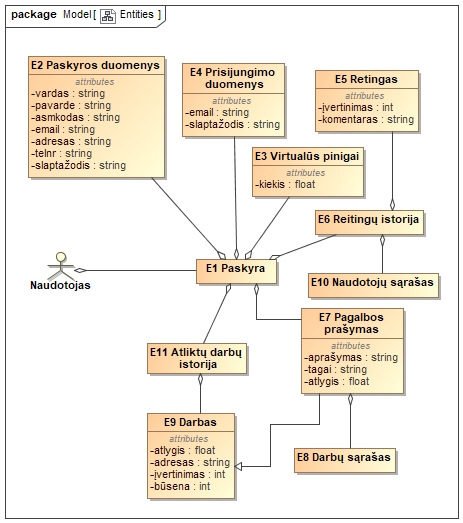
\includegraphics[scale=0.7]{img/Entities}
	\caption{Esybių diagrama}
	\label{img:entities}
\end{figure}
1 pav. vaizduojama sistemos esybių diagrama.

\begin{figure}[H]
	\centering
	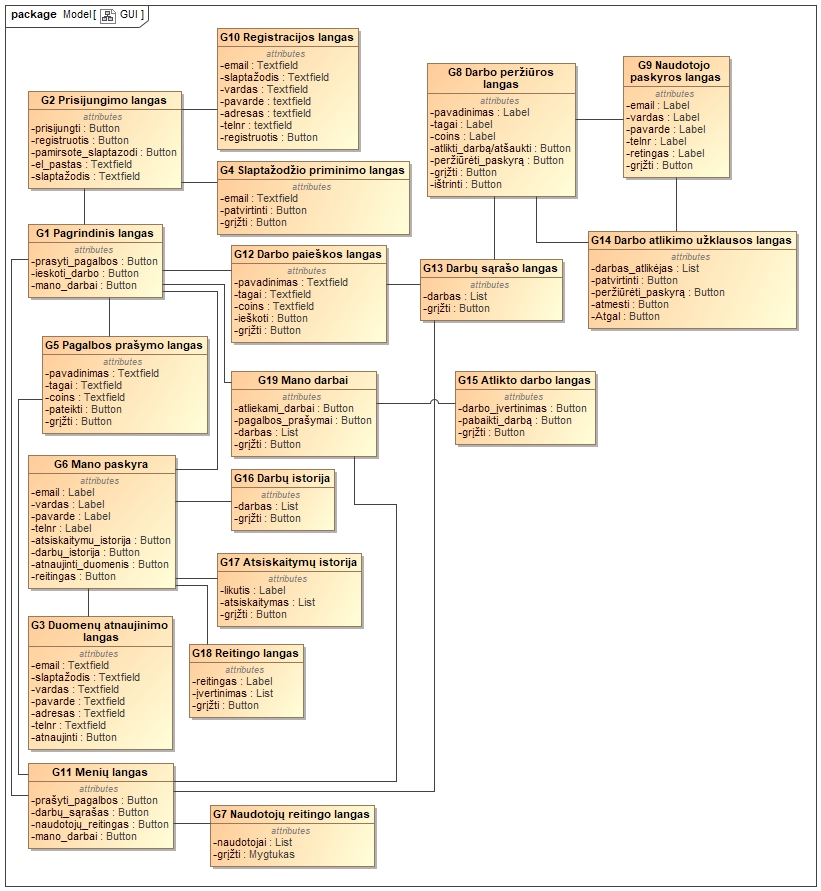
\includegraphics[scale=0.7]{img/GUI}
	\caption{Grafinės sąsajos elementų diagrama}
	\label{img:gui}
\end{figure}
2 pav. vaizduojama grafinės sąsajos elementų diagrama. 

\begin{table}[H]\footnotesize
	\centering
	\caption{Struktūrinio dalykinės srities modelio elementai}
	{\rowcolors{2}{yellow!50}{yellow!40}
	\setlength{\arrayrulewidth}{0.25mm}
	{\begin{tabular}{|c|m{5.75cm}|m{5.75cm}|} \hline
		Kodas & Elementas & Aprašymas \\
		\hline
		\textbf{E1} & Paskyra & Naudotojo paskyra \\
		\textbf{E2} & Registracijos duomenys & Duomenys reikalingi naudotojui registruojantis prie sistemos \\
		\textbf{E3} & Virtualūs pinigai & Virtuali valiuta naudojama atsiskaityti už įvykdytus darbus \\
		\textbf{E4} & Prisijungimo duomenys & Duomenys reikalingi naudotojo autentifikavimui prisijungimo metu \\
		\textbf{E5} & Reitingas & Naudotojo įvertinimas \\
		\textbf{E6} & Reitingų istorija & Naudotojo reitingo kitimo istorija \\
		\textbf{E7} & Pagalbos prašymas & Naudotojo pateikta užduotis, už kurią jis yra pasirįžęs sumokėti pasirinktą virtualių pinigų sumą \\
		\textbf{E8} & Darbų sąrašas & Visų naudotojų pateiktų pagalbos prašymų sąrašas \\
		\textbf{E9} & Darbas & Pagalbos prašymas \\
		\textbf{E10} & Atliekamas darbas & Naudotojo pasirinktas atlikti darbas \\
		\textbf{E11} & Atliktas darbas & Naudotojo atliktas darbas \\
		\textbf{E12} & Atliktų darbų istorija & Visų naudotojo atliktų darbų sąrašas \\
		\hline
		\textbf{G1} & Pagrindinis langas & Langas matomas naudotojui prisijungus prie savo paskyros \\
		\textbf{G2} & Prisijungimo langas & Langas matomas naudotojui įsijungus aplikaciją, naudojamas identifikuoti naudotoją \\
		\textbf{G3} & Paskyros atnaujinimo langas & Langas naudojamas naudotojo paskyros duomenų atnaujinimui \\
		\textbf{G4} & Slaptažodžio priminimo langas & Langas matomas, kai naudotojas prisijungimo metu užmiršta savo slaptažodį \\
		\textbf{G5} & Pagalbos prašymo užpildymo langas & Langas skirtas naudotojo pagalbos prašymui \\
		\textbf{G6} & Mano Paskyra & Langas kuriame naudotojas mato savo paskyros duomenis \\
		\textbf{G7} & Visų naudotojų reitingas & Langas kuriame matomas visų naudotojų reitingų sąrašas \\
		\textbf{G8} & Darbų peržiūros langas & Langas kuriame matomas darbų sąrašas \\
		\textbf{G9} & Kito naudotojo paskyros langas & Langas kuriame naudotojas mato kito naudotojo paskyros informaciją \\
		\hline
	\end{tabular}}
	}
	\label{tab:entity table}
\end{table}

\subsection{Esybių - Užduočių atsekamumo matrica}
Šiame poskyryje pateikiama esybių atsekamumo matrica, kurioje esybės siejamos su funkciniais reikalavimais.
\begin{figure}[H]
    \centering
    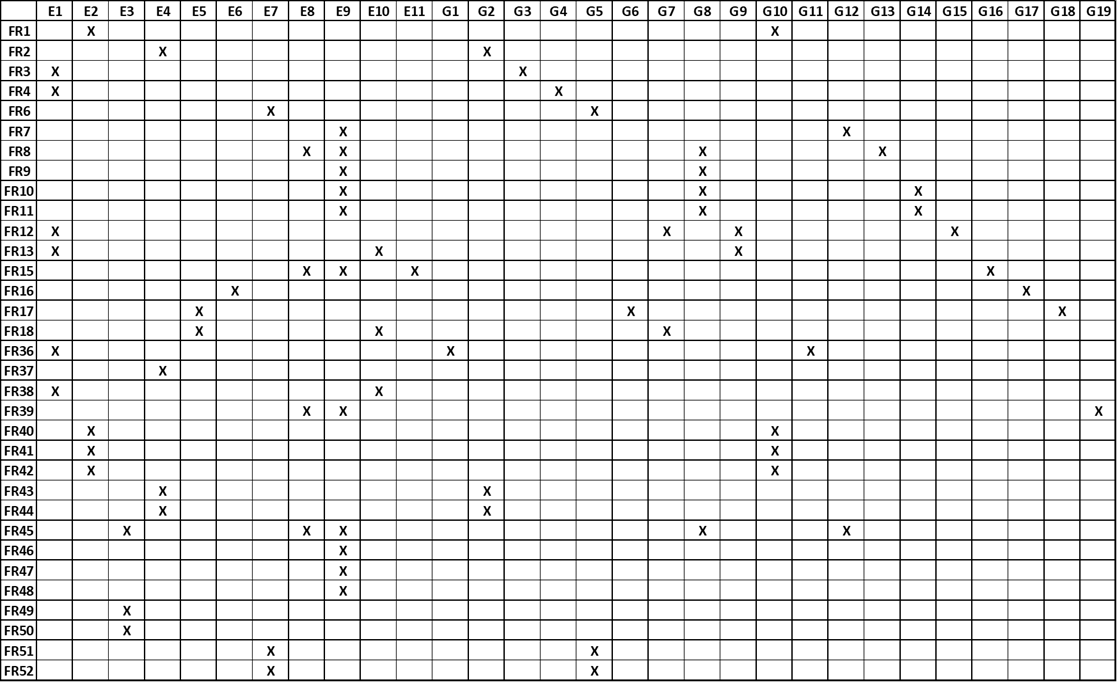
\includegraphics[scale=0.8]{img/Entity-matrix}
    \caption{Esybių-Reikalavimų atsekamumo matrica}
    \label{img:entity-matrix}
\end{figure}

\section{Užduotys}
Šiame skyriuje pateikiamos sistemos užduotys. Aprašomi pagrindiniai ir alternatyvūs jų atlikimo scenarijai.
\begin{figure}[H]
	\centering
	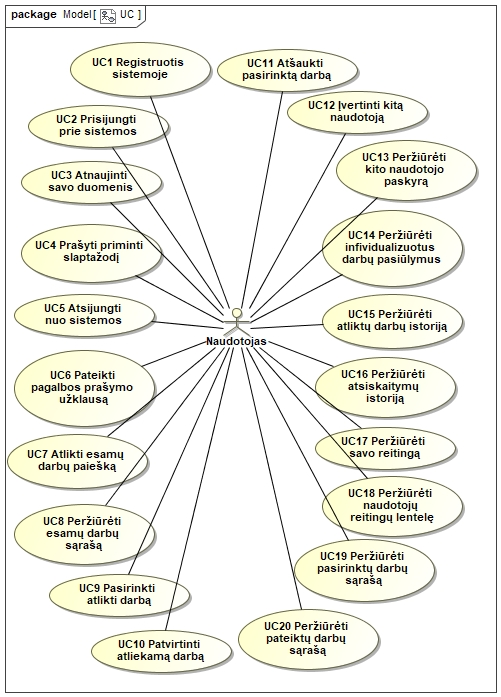
\includegraphics[scale=0.8]{img/UC}
	\caption{Naudotojo užduočių diagrama}
	\label{img:uc}
\end{figure}

\subsection{Naudotojo sąsajos užduotys}
Šiame poskyryje aprašomi naudotojo sąsajos užduočių pagrindiniai ir alternatyvūs scenarijai.

\begin{figure}[H]
	\centering
	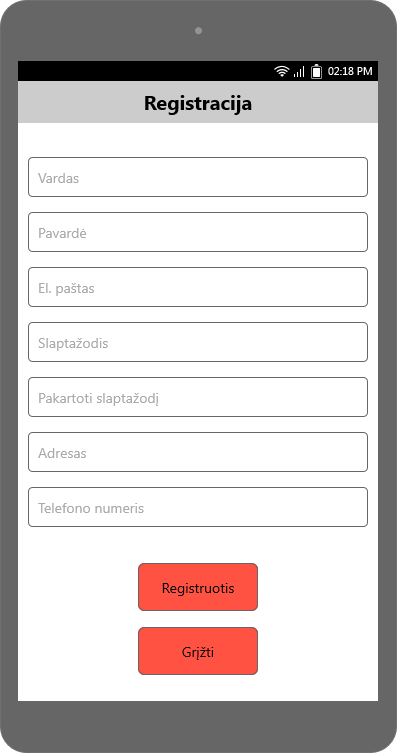
\includegraphics[scale=0.4]{img/ScreenShots/02-Registracijos-langas}
	\caption{Registracijos langas}
	\label{img:reg}
\end{figure}
\subsubsection{UC1 „Registruotis sistemoje“}
\textbf{Pagrindinis scenarijus}. Naudotojas prisijungimo lange spaudžia „Registruotis“, atsiveria registracijos langas. Jame naudotojas į atskirus laukelius suveda registracijos duomenis: el. pašto adresą, slaptažodį, vardą, pavardę, gyvenamosios vietos adresą, telefono numerį bei pakartotinai įveda saptažodį. Viską suvedęs, naudotojas spaudžia „Registruotis“. Tada sistema patikrina, ar suvesti slaptažodžiai sutampa. Jei sutampa, sistema patikrina, ar duomenų bazėje neegzistuoja naudotojas su tokiais duomenimis. Jei ne, sistema siunčia registracijos duomenis į sistemos duomenų bazę ir atveria pagrindinį langą.
\par \textbf{Alternatyvus scenarijus}: naudotojo įvesti slaptažodžiai nesutampa. Tada sistema parodo naudotojui pranešimą, kad įvesti slaptažodžiai nesutampa ir atvaizduoja registracijos langą.
\par \textbf{Alternatyvus scenarijus}: toks naudotojas jau egzistuoja. Tada sistema parodo naudotojui pranešimą, kad toks naudotojas jau egzistuoja ir atvaizduoja pradinį langą.

\begin{figure}[H]
	\centering
	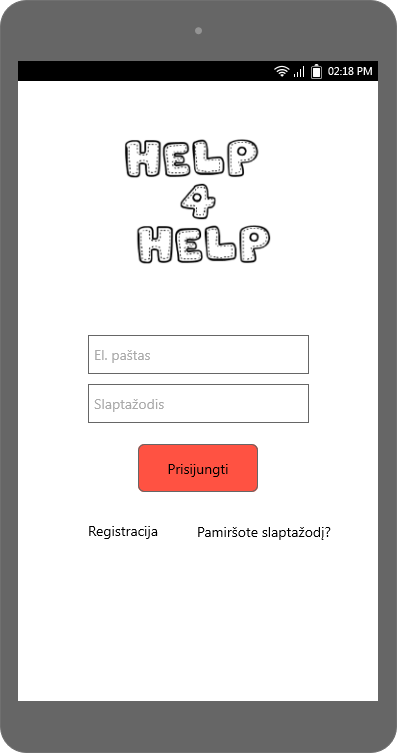
\includegraphics[scale=0.4]{img/ScreenShots/01-Pradinis-langas}
	\caption{Pradinis langas}
	\label{img:login}
\end{figure}
\subsubsection{UC2 „Prisijungti prie sistemos“}
\textbf{Pagrindinis scenarijus}. Pradiniame lange naudotojas suveda prisijungimo duomenis: el. pašto adresą bei slaptažodį. Suvedęs duomenis naudotojas spaudžia „Prisijungti“, tada sistema patikrina, ar įvesti duomenys teisingi. Jei duomenys suvesti teisingai, atsidaro pagrindinis langas.
\par \textbf{Alternatyvus scenarijus}: naudotojas pradiniame lange neteisingai įveda prisijungimo duomenis, tada sistema praneša naudotojui, kad įvesti neteisingi duomenys bei atvaizduoja pradinį langą, kad naudotojas galėtų bandyti prisijungti dar kartą.

\begin{figure}[H]
	\centering
	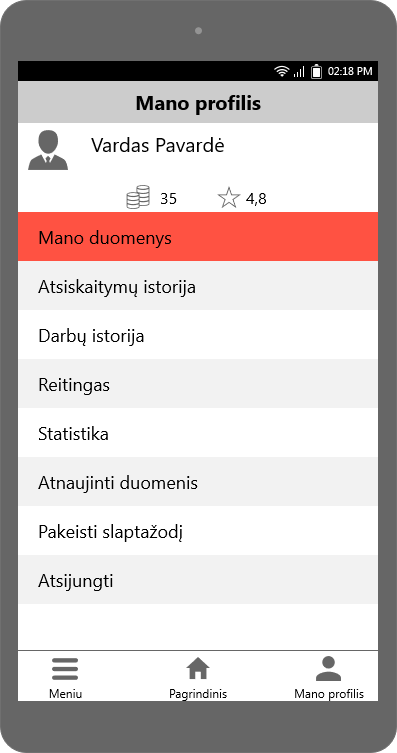
\includegraphics[scale=0.4]{img/ScreenShots/Mano_profilis/00-Mano-profilis}
	\caption{Mano profilis}
	\label{img:profile}
\end{figure}

\begin{figure}[H]
	\centering
	\includegraphics[scale=0.4]{img/ScreenShots/Mano_profilis/03-Duomenų-atnaujinimas}
	\caption{Duomenų atnaujinimo langas}
	\label{img:update profile}
\end{figure}
\subsubsection{UC3 „Atnaujinti savo duomenis“}
\textbf{Pagrindinis scenarijus}. Naudotojas lange „Mano paskyra“ spaudžia „Atnaujinti duomenis“, tada atveriamas duomenų atnaujinimo langas, kuriame vaizduojami esami paskyros duomenys. Esamus paskyros duomenis naudotojas redaguoja ir baigęs redaguoti spaudžia „Išsaugoti pakeitimus“. Tada sistema patikrina, ar įvestas validus el. pašto adresas. Jei taip, sistema atnaujina duomenis duomenų bazėje ir praneša naudotojui, kad duomenys atnaujinti sėkmingai. Tada sistema atvaizduoja langą „Mano paskyra“ su atnaujintais duomenimis. 
\par\textbf{Alternatyvus scenarijus}: naudotojas duomenų atnaujinimo lange suveda netinkamą el. pašto adresą, tada sistema praneša naudotojui, kad įvestas el. paštas yra netinkamas, ir atvaizduoja duomenų atnaujinimo langą.

\begin{figure}[H]
	\centering
	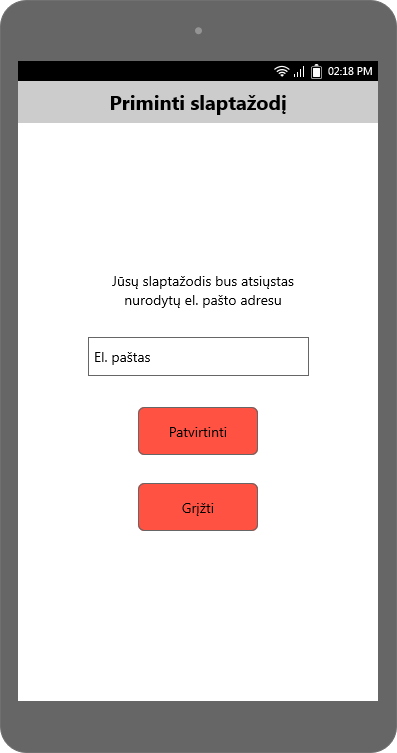
\includegraphics[scale=0.4]{img/ScreenShots/03-Slaptažodžio-priminimo-langas}
	\caption{Slaptažodžio priminimo langas}
	\label{img:forget pass}
\end{figure}
\subsubsection{UC4 „Prašyti priminti slaptažodį“}
\textbf{Pagrindinis scenarijus}. Naudotojas pradiniame lange spaudžia „Pamiršote slaptažodį?“, tada sistema atvaizduoja slaptažodžio priminimo langą, kuriame naudotojas suveda norimos paskyros el. pašto adresą ir spaudžia „Patvirtinti“, tada sistema patikrina el. pašto adresą ir, jei toks naudotojas(su tokiu el. pašto adresu) egzistuoja duomenų bazėje, išsiunčia šiuo el. pašto adresu priminimo laišką su naudotojo slaptažodžiu. 
\par \textbf{Alternatyvus scenarijus}: naudotojas su tokiu el. pašto adresu neegzistuoja, tada sistema praneša naudotojui, kad tokiu el. paštu registruotos anketos nėra, ir atvaizduoja slaptažodžio priminimo langą, kad naudotojas dar kartą galėtų suvesti el. paštą.
\subsubsection{UC5 „Atsijungti nuo sistemos“}
\textbf{Pagrindinis scenarijus}. Naudotojas lange „Mano paskyra“ spaudžia „Atsijungti“, tada sistema pakeičia naudotojo būseną į „neprisijungęs“ ir atvaizduoja „Pradinį langą“.

\begin{figure}[H]
	\centering
	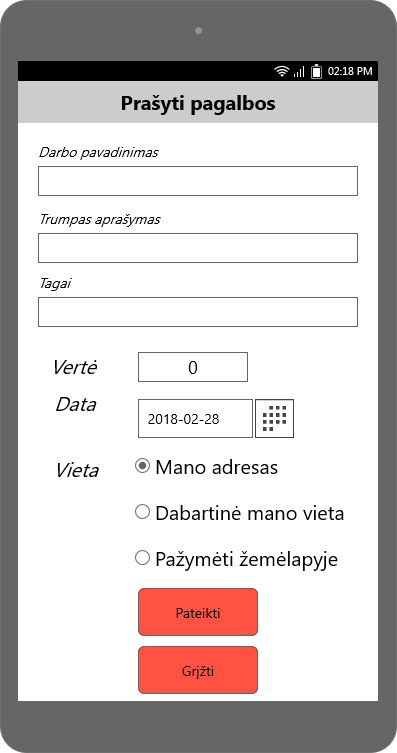
\includegraphics[scale=0.4]{img/ScreenShots/Prašyti_pagalbos/00-Prašyti-pagalbos}
	\caption{Pagalbos prašymo langas}
	\label{img:help}
\end{figure}
\subsubsection{UC6 „Pateikti pagalbos prašymo užklausą“}
\textbf{Pagrindinis scenarijus}. Naudotojas pagrindiniame lange arba šoniniame meniu spaudžia „Prašyti pagalbos“, tada sistema atvaizduoja pagalbos prašymo langą. Naudotojas užpildo prašymą, suvesdamas reikiamus duomenis ir spaudžia „Pateikti“, tada sistema patikrina, ar suvesti duomenys tinkami, ir, jei taip, sukuria naują darbą duomenų bazėje pagal pateiktą prašymą ir praneša naudotojui, kad darbas sukurtas. Tada sistema atvaizduoja pagrindinį langą.
\par \textbf{Alternatyvus scenarijus}: naudotojas suvedė netinkamus duomenis. Tada sistema praneša naudotojui, kad suvesti netinkami duomenys, ir atvaizduoja pagalbos prašymo langą.

\begin{figure}[H]
	\centering
	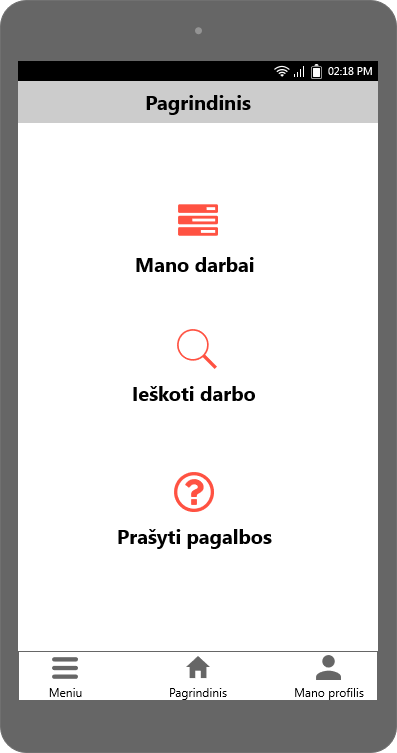
\includegraphics[scale=0.4]{img/ScreenShots/12-Pagrindinis-langas}
	\caption{Pagrindinis langas}
	\label{img:main}
\end{figure}

\begin{figure}[H]
	\centering
	\includegraphics[scale=0.4]{img/ScreenShots/07-Darbo-paieška}
	\caption{Darbo paieškos langas}
	\label{img:find work}
\end{figure}

\begin{figure}[H]
	\centering
	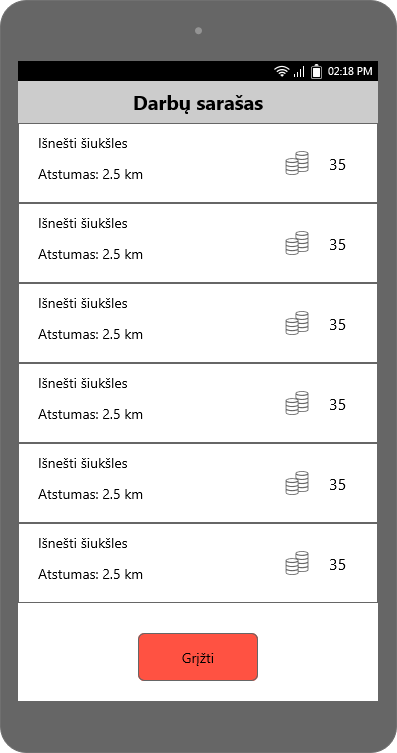
\includegraphics[scale=0.4]{img/ScreenShots/09-Darbų-sąrašas}
	\caption{Darbų sąrašo langas}
	\label{img:work list}
\end{figure}
\subsubsection{UC7 „Atlikti esamų darbų paiešką“}
\textbf{Pagrindinis scenarijus}. Pagrindiniame lange naudotojas spaudžia „Ieškoti darbo“, tada sistema atvaizduoja darbo paieškos langą, tada naudotojas suveda paieškos duomenis ir spaudžia „Ieškoti“, tada sistema suranda visus darbus, atitinkančius tokius paieškos duomenis, ir atvaizduoja šių darbų sąrašą darbų sąrašo lange. 
\par \textbf{Alternatyvus scenarijus}: naudotojas suveda paieškos duomenis ir spaudžia „Ieškoti“, tada sistema duomenų bazėje neranda paieškos duomenis atitinkančių darbų ir praneša naudotojui, kad nėra darbų, atitinkančių pateiktus paieškos duomenis, ir atvaizduoja darbų sąrašo langą su visais esamais darbais.
\subsubsection{UC8 „Peržiūrėti esamų darbų sąrašą“}
\textbf{Pagrindinis scenarijus}. Prisijungęs naudotojas meniu lange spaudžia „Darbų sąrašas“, tada sistema įkelia darbus iš DB, jei rasta daugiau nei 0 darbų, sistema atvaizduoja darbų sąrašo langą, kuriame vaizduojami visi esami darbai.
\par \textbf{Alternatyvus scenarijus}: sistema DB neranda darbų. Tada sistema praneša vartotojui, kad nepavyko rasti darbų ir atvaizduoja tuščią darbų sąrašo langą.

\begin{figure}[H]
	\centering
	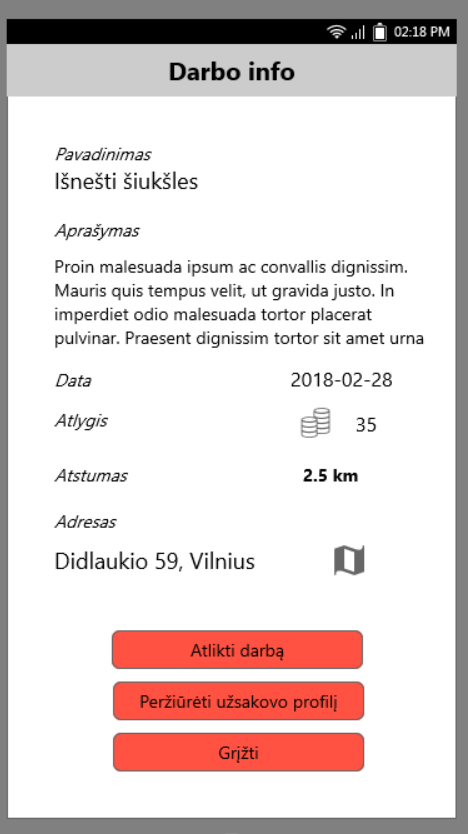
\includegraphics[scale=0.4]{img/ScreenShots/6}
	\caption{Darbo peržiūros langas}
	\label{img:selected job 1}
\end{figure}
\subsubsection{UC9 „Pasirinkti atlikti darbą“}
\textbf{Pagrindinis scenarijus}. Darbo peržiūros lange naudotojas spaudžia „Atlikti darbą“, tada sistema siunčia darbo atlikimo užklausą darbą pateikusiajam naudotojui, o darbą pasirinkusiam naudotojui sistema praneša, kad laukiama darbą pateikusiojo patvirtinimo ir atvaizduoja darbo peržiūros langą, kuriame mygtukas „Atlikti darbą“ pakeistas į „Atšaukti“.

\begin{figure}[H]
	\centering
	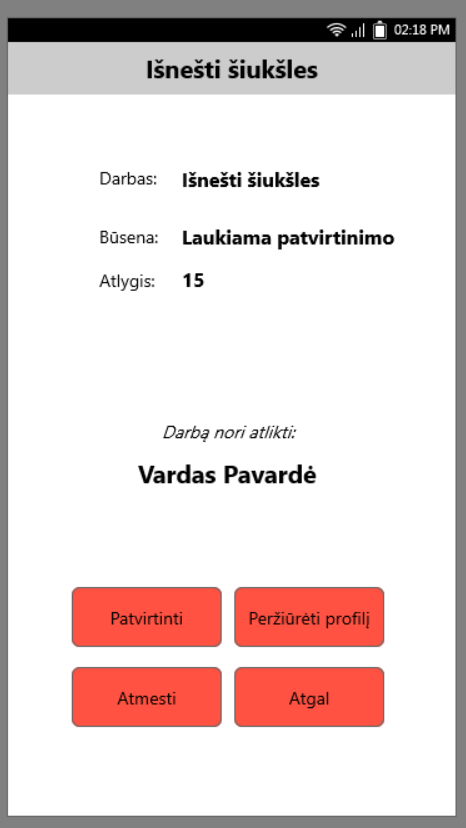
\includegraphics[scale=0.4]{img/ScreenShots/2}
	\caption{Darbo atlikimo užklausos langas}
	\label{img:selected job 2}
\end{figure}
\subsubsection{UC10 „Patvirtinti atliekamą darbą“}
\textbf{Pagrindinis scenarijus}. Naudotojas, gavęs darbo atlikimo užklausą, darbo atlikimo užklausos lange spaudžia „Patvirtinti“, tada sistema siunčia pranešimą darbą pasirinkusiajam naudotojui, pakeičia darbo būseną duomenų bazėje, paskiria darbą pasirinkusį naudotoją tą darbą atliekančiuoju ir atvaizduoja darbo peržiūros langą. 
\par \textbf{Alternatyvus scenarijus}: naudotojas, gavęs darbo atlikimo užklausą, darbo atlikimo užklausos lange spaudžia „Atmesti“, tada sistema darbą pasirinkusiajam naudotojui parodo pranešimą, kad darbo atlikimo užklausa atmesta. Darbo būsena duomenų bazėje nekeičiama.
\subsubsection{UC11 „Atšaukti pasirinktą darbą“}
Naudotojas „Darbo peržiūros lange“ spaudžia „Atšaukti“, tada sistema pakeičia darbo būseną duomenų bazėje bei praneša darbą pateikusiajam, kad darbo atlikimas buvo atšauktas.
\subsubsection{UC12 „Įvertinti kitą naudotoją“}
Naudotojas „Atlikto darbo lange“ pasirenka atlikto darbo įvertinimą iš galimų variantų ir spaudžia „Įvertinti“, tada sistema pasirinktą įvertinimą įveda į duomenų bazę.
\subsubsection{UC13 „Peržiūrėti kito naudotojo paskyrą“}
1. „Darbo peržiūros lange“ naudotojas spaudžia ant darbą pateikusiojo naudotojo vardo, tada sistema atvaizduoja darbą pateikusiojo naudotojo paskyros langą.
2. „Naudotojų reitingo lange“ naudotojas spaudžia ant pasirinkto naudotojo vardo, tada sistema atvaizduoja darbą pateikusiojo naudotojo paskyros langą.

\begin{figure}[H]
	\centering
	\includegraphics[scale=0.4]{img/ScreenShots/Mano_profilis/07-Darbų-istorija}
	\caption{Darbų istorijos langas}
	\label{img:work history}
\end{figure}
\subsubsection{UC14 „Peržiūrėti atliktų darbų istoriją“}
Naudotojas šoniniame meniu spaudžia „Mano darbai“, tada sistema atvaizduoja langą „Mano darbai“, tada naudotojas spaudžia „Atliekami darbai“, tada sistema atvaizduoja langą „Mano darbai 2“, kuriame pateikiami naudotojo pasirinkti atlikti, atliekami bei atlikti darbai.

\begin{figure}[H]
	\centering
	\includegraphics[scale=0.4]{img/ScreenShots/Mano_profilis/05-Atsiskaitymų-istorija}
	\caption{Atsiskaitymų istorijos langas}
	\label{img:payment history}
\end{figure}
\subsubsection{UC15 „Peržiūrėti atsiskaitymų istorija“}
Naudotojas lange „Mano profilis“ spaudžia „Atsiskaitymų istorija“, tada sistema atvaizduoja langą „Atsiskaitymų istorija“, kuriame pateikiami visi atsiskaitymai už atliktus darbus.

\begin{figure}[H]
	\centering
	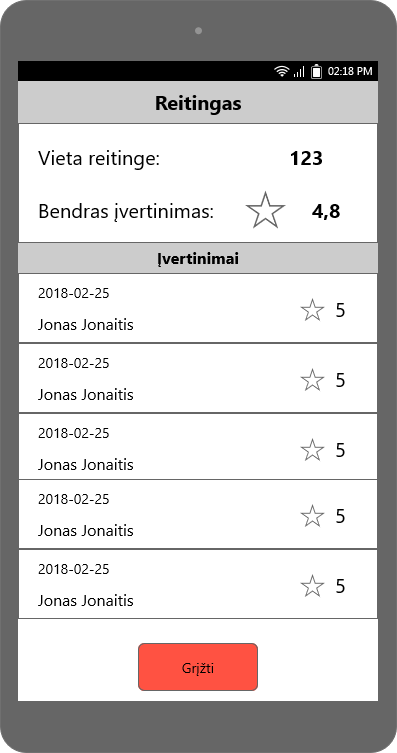
\includegraphics[scale=0.4]{img/ScreenShots/Mano_profilis/06-Reitingas}
	\caption{Reitingo langas}
	\label{img:rating}
\end{figure}
\subsubsection{UC16 „Peržiūrėti savo reitingą“}
1. Naudotojas lange „Mano profilis“ mato savo reitingą. \\
2. Naudotojas lange „Mano profilis“ spaudžia „Reitingas“, tada sistema atvaizduoja langą „Reitingas“, kuriame pateikti visi gauti įvertinimai bei įvertinimų vidurkis(reitingas).

\begin{figure}[H]
	\centering
	\includegraphics[scale=0.4]{img/ScreenShots/10-Naudotojų-reitingas}
	\caption{Visų naudotojų reitingų lentelė}
	\label{img:rating table}
\end{figure}
\subsubsection{UC17 „Peržiūrėti naudotojų reitingų lentelę“}
Naudotojas šoniniame meniu spaudžia „Naudotojų reitingas“, tada sistema atvaizduoja „Naudotojų reitingo“ langą, kuriame pateikiamas visų naudotojų sąrašas surikiuotas pagal reitingą.

\begin{figure}[H]
	\centering
	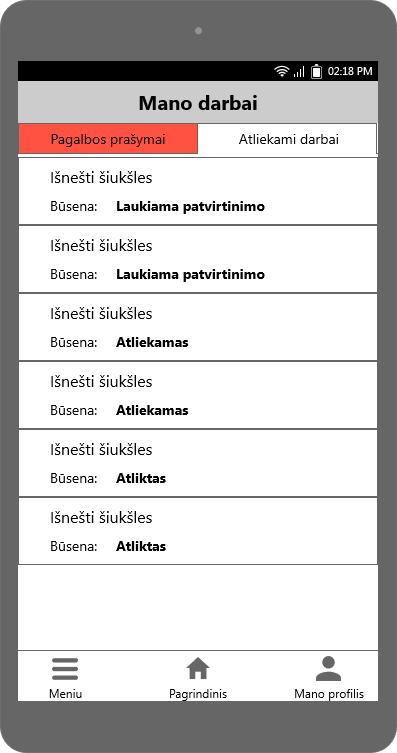
\includegraphics[scale=0.4]{img/ScreenShots/06-Mano-darbai2}
	\caption{Pasirinktų darbų lentelė}
	\label{img:selected jobs table}
\end{figure}
\subsubsection{UC18 „Peržiūrėti pasirinktų darbų sąrašą“}
Naudotojas šoniniame meniu arba „Pagrindiniame lange“ spaudžia „Mano darbai“, tada sistema atvaizduoja langą „Mano darbai 1“, tada naudotojas spaudžia „Atliekami darbai“, tada sistema atvaizduoja langą „Mano darbai 2“, kuriame pateikiamas naudotojo pasirinktų darbų sąrašas.

\begin{figure}[H]
	\centering
	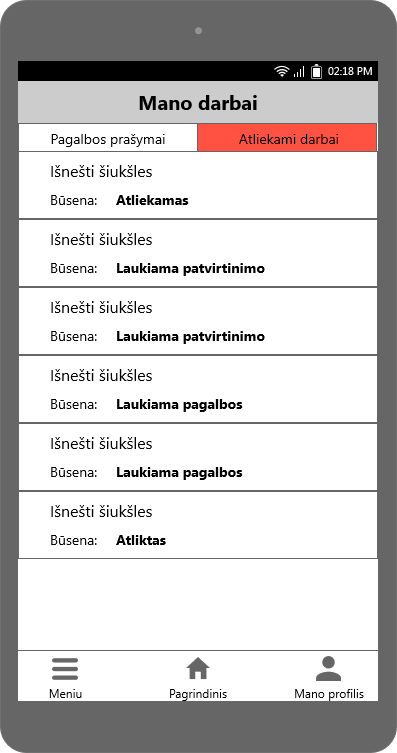
\includegraphics[scale=0.4]{img/ScreenShots/05-Mano-darbai1}
	\caption{Pasirinktų darbų lentelė}
	\label{img:requested jobs table}
\end{figure}
\subsubsection{UC19 „Peržiūrėti pateiktų darbų sąrašą“}
Naudotojas šoniniame meniu arba „Pagrindiniame lange“ spaudžia „Mano darbai“, tada sistema atvaizduoja langą „Mano darbai 1“, kuriame pateikiamas naudotojo pateiktų darbų sąrašas.
\subsubsection{UC20 „Ištrinti pateiktą darbą“}
Naudotojas „Darbo peržiūros lange“ spaudžia „Ištrinti“, tada sistema perklausia naudotojo, ar tikrai jis nori ištrinti pateiktą darbą, tada naudotojas spaudžia „Taip“, tada sistema patikrina, ar darbo nėra pasirinkęs, ar nėra pradėjęs vykdyti kitą naudotojas. Jei nėra, tai sistema ištrina darbą iš duomenų bazės ir praneša naudotojui, kad darbą pašalintas sėkmingai.
\textbf{Alternatyvūs scenarijai}: \\
1. Naudotojo norimą ištrinti darbą yra pasirinkęs atlikti kitas naudotojas, tada sistema praneša darbą ištrinti norinčiam naudotojui, kad pirmiausiai reikia atšaukti darbo atlikimo užklausą, o tada galima ištrinti darbą. Tada sistema atvaizduoja „Darbo peržiūros langą“.\\ 
2. Naudotojo norimą ištrinti darbą jau atlieka kitas naudotojas, tada sistema praneša darbą ištrinti norinčiam naudotojui, kad darbo ištrinti negalima, nes jis jau yra atliekamas, ir atvaizduoja „Darbo peržiūros langą“.
\subsection{Reikalavimų - Užduočių atsekamumo matrica}
Šiame poskyryje pateikiama užduočių atsekamumo matrica, kurioje užduotys siejamos su funkciniais reikalavimais.
\begin{figure}[H]
    \centering
    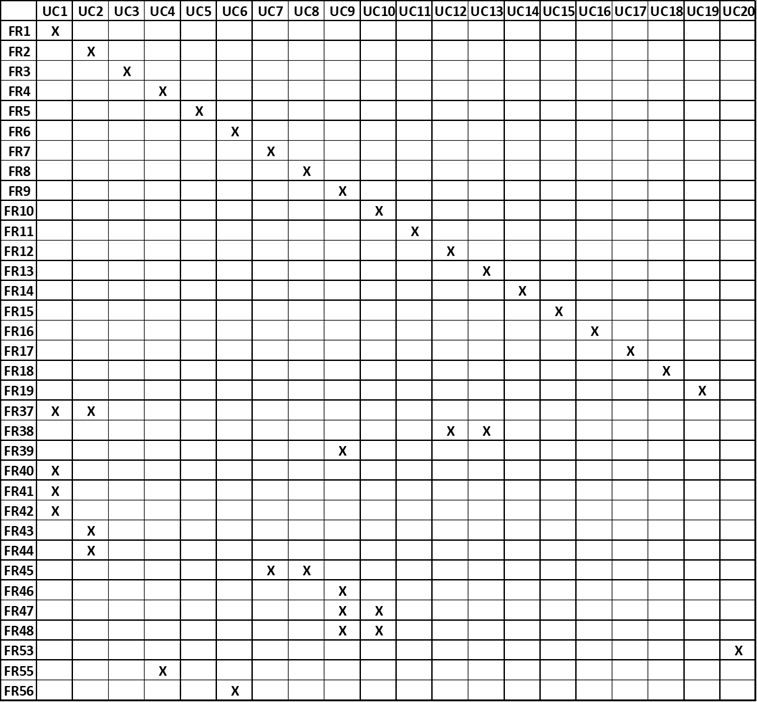
\includegraphics[scale=0.8]{img/UC-matrix}
    \caption{Užduočių-Reikalavimų atsekamumo matrica}
    \label{img:uc-matrix}
\end{figure}

\sectionnonum{Išvados}
Remiantis ICONIX procesu, buvo peržiūrėti ir šiame dokumente surašyti visi reikalavimai mobiliajai programėlei „Help4Help". Taip pat sukurtas ir pateiktas dalykinės srities modelis bei naudotojo užduočių diagrama, aprašyti užduočių vykdymo scenarijai bei sukurtos atsekamumo matricos.

\printbibliography[heading=bibintoc]  % Šaltinių sąraše nurodoma panaudota
% literatūra, kitokie šaltiniai. Abėcėlės tvarka išdėstomi darbe panaudotų
% (cituotų, perfrazuotų ar bent paminėtų) mokslo leidinių, kitokių publikacijų
% bibliografiniai aprašai. Šaltinių sąrašas spausdinamas iš naujo puslapio.
% Aprašai pateikiami netransliteruoti. Šaltinių sąraše negali būti tokių
% šaltinių, kurie nebuvo paminėti tekste. Šaltinių sąraše rekomenduojame
% necituoti savo kursinio darbo, nes tai nėra oficialus literatūros šaltinis.
% Jei tokių nuorodų reikia, pateikti jas tekste.

% Priedai
\appendix
\section{Rastos klaidos ir jų sprendimai}
\begin{table}[H]\footnotesize
	\centering
	\caption{Klaidos}
	{\rowcolors{2}{yellow!50}{yellow!40}
	\setlength{\arrayrulewidth}{0.25mm}
	{\begin{tabular}{|c|m{5.75cm}|m{5.75cm}|} \hline
		Kodas & Klaida & Sprendimas \\
		\hline
		\textbf{K1} & Sistemos realizavimas pririštas prie specifinio OS & Pakeisti reikalavimą \\
		\textbf{K2} & Aplikacija kuriama C\# programavimo kalba naudojant Visual Studio & Kalbą pakeisti į Java, o IDE į Android Studio \\
		\textbf{K3} & Aplikacija turi pranešti apie atnaujinimus 12 valandų prieš jų išėjimą & Aplikacija vartotojui praneš tik išėjus atnaujinimams \\
		\textbf{K4} & Registracijai reikalingas asmens kodas ir gyvenamosios vietos adresas & Nereikalauti asmens kodo ir gyvenamosios vietos adreso registracijos metu \\
		\textbf{K5} & Naudotojui užmiršus slaptažodį, jis jį turėjo būtinai pakeisti & Naudotojui užmiršus slaptažodį, jis gali prašyti jį priminti \\
		\hline
	\end{tabular}}
	}
	\label{tab:mistake table}
\end{table}

\section{Žodynas}
\begin{table}[H]\footnotesize
	\centering
	\caption{Terminų žodynas}
	{\rowcolors{2}{yellow!50}{yellow!40}
	\setlength{\arrayrulewidth}{0.25mm}
	{\begin{tabular}{|c|c|m{11.5cm}|} \hline
		Kodas & Terminas & Reikšmė \\
		\hline
		\textbf{T1} & Naudotojas & Fizinis asmuo, kuris turi paskyrą aplikacijoje, kurios dėka gali pateikti pagalbos prašymą ar pagalbą suteikt \\
		\textbf{T2} & Pagalbos prašantysis & Mobilios aplikacijos naudotojas, kuris išsikviečia pagalbą \\
		\textbf{T3} & Pagalbos teikėjas & Mobilios aplikacijos naudotojas, kuris  priima pagalbos prašymą ir atlieka darbą \\
		\textbf{T4} & Administratorius & Fizinis asmuo, turintis išskirtines teises sistemoje, prižiūri sąžiningą darbų atlikimą ir atsiskaitymą. Nesilaikančius taisyklių vartotojus gali užblokuoti \\
		\textbf{T5} & Pagalbos prašymas & Užklausa aplikacijoje, kurią naudotojas pateikia sistemai pagal sistemoje nurodytą procedūrą, ir kurioje tiesiogiai nurodomas norimos pagalbos pobūdis \\
		\textbf{T6} & Atsiskaitymas & Pagalbos prašytojo pervedama taškų/kreditų suma už atlikta darbą/paslaugą \\
		\hline
	\end{tabular}}
	}
	\label{tab:dictionary}
\end{table}
	


\end{document}

%Skyrių ir poskyrių pavyzdys
%\section{Skyrius}
%\subsection {Poskyris}
%\subsubsection {Skirsnis}
%\subsubsubsection {Straipsnis}
%Tekstas

%\sectionnonum{Nenumeruojamas skyrius}
